%-----------------------------------------------------------------------------------------
\clearpage
\section{Project Plan and Time Management}
%-----------------------------------------------------------------------------------------
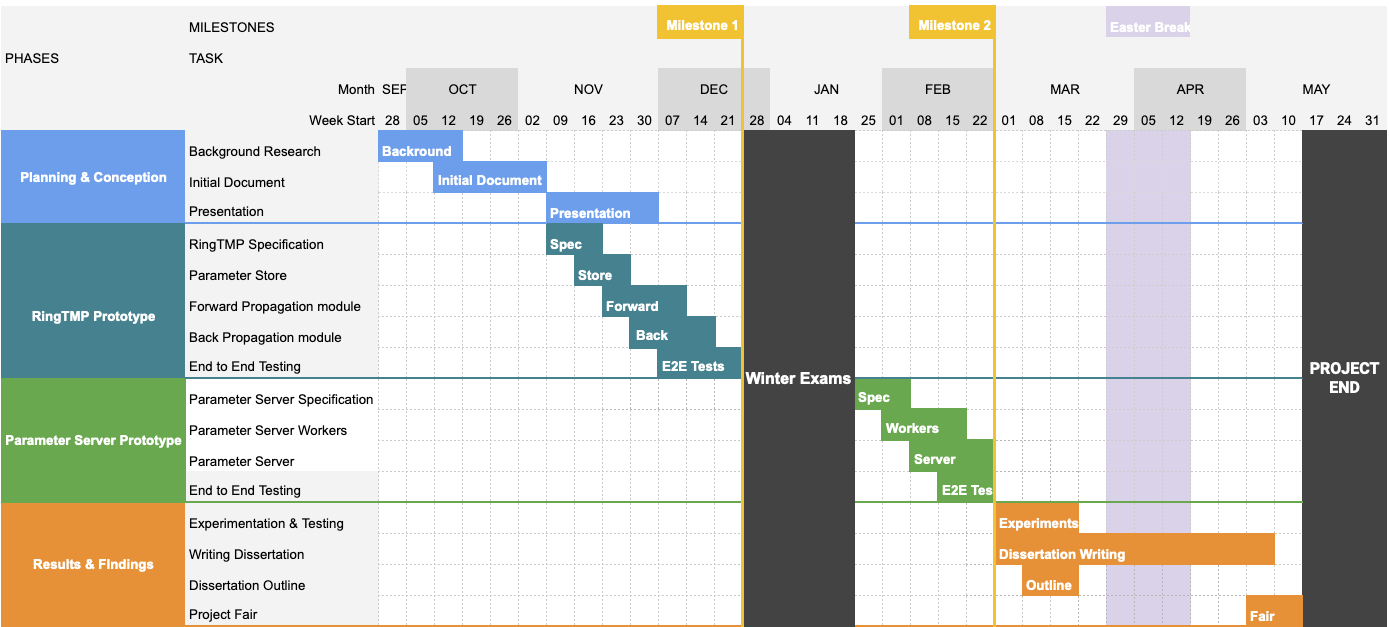
\includegraphics[width=16cm, height=8cm]{BetterGant.png}

The gant chart above outlines the order and time frame each task should take in
order complete this dissertation on time and to a high quality. After
researching the background and submitting the initial document. Building a
RingTMP prototype of my system is the most important task to embark on. It is
better to do this first as it will take the longest time to produce and has the
most 'unknown unknowns', moreover this is the centrepiece of my project if I
have not finished this there will be no dissertation to write. I then take a
month break to revise for my exams. I acknowledge that this is a long time,
however semester 1 modules contribute more to my final grade than my
dissertation does, therefore its important this project isn't detrimental to my
grades in other modules. After Christmas I'll start work on a basic prototype of
a parameter server. This will use the same tools and languages as my framework.
In this way it will be easy to compare and contrast the benefits and
shortcomings of each system on a level playing field. Once Both pieces of
software have been complete I will run various tests to see how well my aims
have been achieved. While I'm conducting these tests I shall also be writing up
my results. Once my experiments have finished I shall start working on my
dissertation document in earnest. I'll hand in my outline a week before easter
break and shall keep working till it is complete, hopefully sometime before the
project deadline (TBC) sometime in May.

\subsection{Applied Methodology}

My project lends itself to using an experimental research methodology to collect
my findings, with this in mind is paramount to ensure that my results are taken
is as controlled conditions as possible

